\documentclass[authoryear, 12pt, a4paper]{elsarticle}

% ------------ packages -------------

\usepackage[utf8]{inputenc}
\usepackage[OT1]{fontenc}
\usepackage{graphicx}
\usepackage[english]{babel}

\usepackage{amsmath}
\usepackage{amsfonts}
\usepackage{amssymb}
\usepackage{amsthm}

\usepackage[usenames,dvipsnames]{xcolor}
\usepackage{todonotes}
\usepackage{etoolbox}
\usepackage{url}
%\usepackage{tikz}
%\usetikzlibrary{shapes.misc,fit}

\usepackage[bookmarks]{hyperref}

% ------------ custom defs -------------

\newcommand{\reals}{\mathbb{R}}
\newcommand{\posreals}{\reals_{>0}}
\newcommand{\posrealszero}{\reals_{\ge 0}}
\newcommand{\naturals}{\mathbb{N}}

\newcommand{\mbf}[1]{\mathbf{#1}}
\newcommand{\bs}[1]{\boldsymbol{#1}}
\renewcommand{\vec}[1]{{\bs#1}}

\newcommand{\uz}{^{(0)}} % upper zero
\newcommand{\un}{^{(n)}} % upper n
\newcommand{\ui}{^{(i)}} % upper i

\newcommand{\ul}[1]{\underline{#1}}
\newcommand{\ol}[1]{\overline{#1}}

\newcommand{\Rsys}{R_\text{sys}}
\newcommand{\lRsys}{\ul{R}_\text{sys}}
\newcommand{\uRsys}{\ol{R}_\text{sys}}

\newcommand{\Fsys}{F_\text{sys}}
\newcommand{\lFsys}{\ul{F}_\text{sys}}
\newcommand{\uFsys}{\ol{F}_\text{sys}}

\def\Tsys{T_\text{sys}}

\newcommand{\E}{\operatorname{E}}
\newcommand{\V}{\operatorname{Var}}

\newcommand{\indic}{\mathbb{I}}

\newcommand{\ber}{\operatorname{Bernoulli}} 
\newcommand{\bin}{\operatorname{Binomial}}
\newcommand{\be}{\operatorname{Beta}} 
\newcommand{\bebin}{\operatorname{Beta-binomial}} 

\def\tmax{t_\text{max}}
\def\tnow{t_\text{now}}
\def\tpnow{t^+_\text{now}}

\def\yz{y\uz}
\def\yn{y\un}
%\def\yi{y\ui}
\newcommand{\yfun}[1]{y^{({#1})}}
\newcommand{\yfunl}[1]{\ul{y}^{({#1})}}
\newcommand{\yfunu}[1]{\ol{y}^{({#1})}}

\def\yl{\ul{y}}
\def\yu{\ol{y}}
\def\nl{\ul{n}}
\def\nu{\ol{n}}
\def\nktzo{\widetilde{n}\uz_{k,t}}

\def\ykt{y_{k,t}}

\def\ykz{y\uz_k}
\def\ykn{y\un_k}

\def\yktz{y\uz_{k,t}}
\def\yktn{y\un_{k,t}}

\def\yzl{\ul{y}\uz}
\def\yzu{\ol{y}\uz}
\def\ynl{\ul{y}\un}
\def\ynu{\ol{y}\un}
\def\yil{\ul{y}\ui}
\def\yiu{\ol{y}\ui}

\def\ykzl{\ul{y}\uz_k}
\def\ykzu{\ol{y}\uz_k}
\def\yknl{\ul{y}\un_k}
\def\yknu{\ol{y}\un_k}

\def\yktzl{\ul{y}\uz_{k,t}}
\def\yktzu{\ol{y}\uz_{k,t}}
\def\yktnl{\ul{y}\un_{k,t}}
\def\yktnu{\ol{y}\un_{k,t}}

\newcommand{\ytz}[1]{y\uz_{#1,t}}
\newcommand{\ytzl}[1]{\ul{y}\uz_{#1,t}}
\newcommand{\ytzu}[1]{\ol{y}\uz_{#1,t}}

\newcommand{\ytn}[1]{y\un_{#1,t}}
\newcommand{\ytnl}[1]{\ul{y}\un_{#1,t}}
\newcommand{\ytnu}[1]{\ol{y}\un_{#1,t}}

\def\nz{n\uz}
\def\nn{n\un}
%\def\ni{n\ui}
\newcommand{\nfun}[1]{n^{({#1})}}
\newcommand{\nfunl}[1]{\ul{n}^{({#1})}}
\newcommand{\nfunu}[1]{\ol{n}^{({#1})}}

\def\nkz{n\uz_k}
\def\nkn{n\un_k}
\newcommand{\nkzfun}[1]{n\uz_{#1}}

\def\nkt{n_{k,t}}

\def\nktz{n\uz_{k,t}}
\def\nktn{n\un_{k,t}}


\def\nzl{\ul{n}\uz}
\def\nzu{\ol{n}\uz}
\def\nnl{\ul{n}\un}
\def\nnu{\ol{n}\un}
\def\nil{\ul{n}\ui}
\def\niu{\ol{n}\ui}

\def\nkzl{\ul{n}\uz_k}
\def\nkzu{\ol{n}\uz_k}
\def\nknl{\ul{n}\un_k}
\def\nknu{\ol{n}\un_k}

\def\nktzl{\ul{n}\uz_{k,t}}
\def\nktzu{\ol{n}\uz_{k,t}}
\def\nktnl{\ul{n}\un_{k,t}}
\def\nktnu{\ol{n}\un_{k,t}}

\newcommand{\ntz}[1]{n\uz_{#1,t}}
\newcommand{\ntzl}[1]{\ul{n}\uz_{#1,t}}
\newcommand{\ntzu}[1]{\ol{n}\uz_{#1,t}}

\def\taut{\tau(\vec{t})}
\def\ttau{\tilde{\tau}}
\def\ttaut{\ttau(\vec{t})}

\def\MZ{\mathcal{M}\uz}
\def\MN{\mathcal{M}\un}

\def\MkZ{\mathcal{M}\uz_k}
\def\MkN{\mathcal{M}\un_k}

\def\MktZ{\mathcal{M}\uz_{k,t}}
\def\MktN{\mathcal{M}\un_{k,t}}

\def\PZ{\Pi\uz}
\def\PN{\Pi\un}

\def\PkZ{\Pi\uz_k}
\def\PkN{\Pi\un_k}
\newcommand{\PZi}[1]{\Pi\uz_{#1}}

\def\PktZ{\Pi\uz_{k,t}}
\def\PktN{\Pi\un_{k,t}}
\newcommand{\PtZi}[1]{\Pi\uz_{#1,t}}
\newcommand{\PkZi}[1]{\Pi\uz_{k,#1}}



%\newcommand{\comments}[1]{{\small\color{gray} #1}}
\newtoggle{td}
\newcommand{\td}[1]{%
  \iftoggle{td}{%
    \todo[inline]{#1}%
  }{}%
}

% ------------ options -------------

\allowdisplaybreaks

\toggletrue{td} % show todo's
%\togglefalse{td} % hide todo's

%\biboptions{longnamesfirst,angle,semicolon}


\journal{IJAR}

\begin{document}

% ------------ frontmatter -------------

\begin{frontmatter}
\title{Bayesian Nonparametric System Reliability\\ using Sets of Priors}

\author[ein]{Gero Walter\fnref{fn1}}
\ead{g.m.walter@tue.nl}
\author[oxf]{Louis J.M. Aslett}
\ead{louis.aslett@stats.ox.ac.uk}
\author[dur]{Frank P.A. Coolen}
\ead{frank.coolen@durham.ac.uk}

\address[ein]{School of Industrial Engineering, Eindhoven University of Technology, Eindhoven, NL}
\address[oxf]{Department of Statistics, University of Oxford, Oxford, UK}
\address[dur]{Department of Mathematical Sciences, Durham University, Durham, UK}

\fntext[fn1]{Gero Walter was supported by the Dinalog project
``Coordinated Advanced Maintenance and Logistics Planning for the Process Industries'' (CAMPI).}

\begin{abstract}
Imprecise Bayesian nonparametric approach to system reliability with multiple types of components,
sets of priors through sets of canonical parameters,
leading to sets of system reliability functions,
reflection of prior-data conflict
\end{abstract}

\begin{keyword}
System reliability \sep
Survival signature \sep
Imprecise probability \sep
Bayesian Nonparametrics \sep
Prior-data conflict
\end{keyword}
\end{frontmatter}


% ------------ manuscript -------------

(author order to be discussed of course)

\section{Introduction}

(some sentences may be useful for the abstract)

System with components of $k=1,\ldots,K$ different types.
There are $m_k$ components of type $k$ in the system.
Components of the same type are i.i.d.\ and independent of components of other types.
Arbitrary system layout, i.e.\ any series / parallel combination, $k$ out of $n$ etc.

Based on expert assumptions for component failure distribution and component test data,
we make predictive inference for a system with components that are exchangeable
with the test components by calculating the system reliability function $\Rsys(t) = P(\Tsys > t)$.
Considering a discrete grid of time points $\{t_1, \ldots, \tmax\}$,
naturally a Bayesian model for the functioning probability at each time point arises.
To account for uncertainty in the choice of prior and due to the inherent issue with prior-data conflict,
we propose an imprecise or interval probability approach
based on sets of prior distributions defined through sets of canonical parameters.

Our method produces a set of discrete system reliability functions,
or, for each time point $t$, an interval for the system survival probability
that appropriately reflects uncertainty due to vague prior information, the amount of test data, and prior-data conflict.

This paper implements the nonparametric approach described in Section~4 of \citet{2015:bayessurvsign}
and extends it to sets of priors.

\section{Survival Signature}

The survival signature allows for straightforward computation of system reliability
for systems with complex layouts and multiple component types.
It separates the (time-invariant) system structure from the time-dependent failure probabilities of components.

Can be seen as applying the law of total probability by partitioning
according to the number of components of type $k$ functioning at time $t$,
denoted by $C^k_t \in \{0, 1, \ldots, l_k, \ldots, m_k\}$:
\begin{align*}
P(\Tsys > t)
 &= \sum_{l_1=0}^{m_1} \cdots \sum_{l_K=0}^{m_K} P(\Tsys > t \mid C^1_t = l_1,\ldots, C^K_t = l_K)
                                                 P\Big( \bigcap_{k=1}^K \{ C^k_t = l_k\} \Big) \\
 &= \sum_{l_1=0}^{m_1} \cdots \sum_{l_K=0}^{m_K} \Phi(l_1, \ldots, l_K)
                                                 \prod_{k=1}^K P(C^k_t = l_k) \,.
\end{align*}


\section{Nonparametric Bayesian Approach}

The random failure time of component number $i$ of type $k$ is denoted by $T^k_i$, $i = 1, \ldots m_k$.
The failure time distribution can be written in terms of the cdf $F^k(t) = P(T^k_i \le t)$,
or in terms of the reliability function $R^k(t) = P(T^k > t) = 1 - F^k(t)$,
also known as the survival function.
For a nonparametric description of $R^k(t)$,
we consider a set of time points $t$, $t \in {\cal T} = \{t_1, \ldots, \tmax\}$.

For each time point $t$, the functioning of a single component of type $k$ at time $t$ (functioning: 1, failed: 0)
is Bernoulli distributed with a suitable functioning probability (as, $1-$failure probability) $p^k_t$, so
\begin{align*}
P\big(\indic(T^k_i > t) = 1\big) &= p^k_t\,, \\
P\big(\indic(T^k_i > t) = 0\big) &= 1 - p^k_t\,,
\end{align*}
in short, $\indic(T^k_i > t) \sim \ber(p^k_t)$, $i = 1, \ldots, m_k$, $t \in {\cal T}$.

The set of functioning probabilities $\{ p^k_t, t \in {\cal T}\}$
defines a discrete failure time distribution for components of type $k$ through
\begin{align*}
R^k(t_j) &= P(T^k > t_j) = p^k_{t_j},\ t_j = t_1, \ldots, \tmax\,.
\end{align*}
We can express this failure time distribution also through the probability mass function (pmf) and the discrete hazard function,
\begin{align*}
f^k(t_j) &= P\big(T^k \in (t_j,t_{j+1}]\big) = p^k_{t_j} - p^k_{t_{j+1}}\,,\\ 
h^k(t_j) &= P\big(T^k \in (t_j,t_{j+1}]\mid T^k > t_j\big) = \frac{f^k(t_j)}{R^k(t_j)}\,. % or R^k(t_{j-1}) ???
\end{align*}
We assume the time grid $\cal T$ is dense enough for the application at hand,
otherwise it would be possible to assume, e.g.,
$R^k(t) = p^k_{t_j}, t \in [t_j, t_{j+1})$,
or taking $p^k_{t_j}$ and $p^k_{t_{j+1}}$ as upper and lower bounds for $R^k(t)$, $t \in [t_j, t_{j+1})$.

\td{***illustrate discrete distribution with a graph of R, q, h?***}

Due to the independence assumption for components of the same type, 
the number of functioning components out of the $m_k$ components of type $k$
is binomially distributed, $C^k_t = \sum_{i=1}^{m_k} \indic(T^k_i > t) \sim \bin(p^k_t, m_k)$.
%(maybe not relevant for this manuscript, but would it make sense to take Kaplan-Meier estimates for the $p^k_t$'s,
%or the NPI bounds for Kaplan-Meier?)

The $p^k_t$'s can be taken such that they reflect, e.g., a bathtub curve for the corresponding hazard rate $h_k(t)$.
Naturally, $p^k_{t_j} \ge p^k_{t_{j+1}}$ should hold (assuming no repair).

However, directly choosing the $p^k_t$'s is hard,
and fixing values for all $p^k_t$ would furthermore neglect any inherent uncertainty in the particular choice.  
To account for this uncertainty, one can express knowledge on $p^k_t$ through a prior distribution.
A convenient and natural choice is $p^k_t \sim \be(\alpha^k_t, \beta^k_t)$, a conjugate prior,
leading to the posterior being again Beta.

Having observed the lifetime data $\vec{t}^k = (t^k_1, \ldots, t^k_{n_k})$,
at any fixed time $t \in {\cal T}$ this results in the observation from the Binomial model described above,
$s^k_t = \sum_{i=1}^{n_k} \indic(t^k_i > t)$.
The posterior is then $p^k_t \mid s^k_t \sim \be(\alpha^k_t + s^k_t, \beta^k_t + n_k - s^k_t)$.
The combination of a Binomial observation model with a Beta prior is often called Beta-binomial model.

The posterior predictive distribution for the number of components surviving at time $t$
of the $m_k$ components in the system, based on the lifetime data and the prior information,
is then a so-called Beta-binomial distribution,
$C^k_t \mid s^k_t \sim \bebin(m_k, \alpha^k_t + s^k_t, \beta^k_t + n_k - s^k_t)$.
That is, we have
\begin{align*}
P(C^k_t = l_k \mid s^k_t) &= {m_k \choose l_k} \frac{B(l_k + \alpha^k_t + s^k_t, m_k - l_k + \beta^k_t + n_k - s^k_t)}
                                                    {B(\alpha^k_t + s^k_t, \beta^k_t + n_k - s^k_t)} \,,
\end{align*}
where $B(\cdot, \cdot)$ is the Beta function.
This posterior predictive distribution is basically a Binomial distribution
where the functioning probability $p^k_t$ takes values in $[0,1]$
with the probability given by the posterior on $p^k_t$.

To wrap up, to calculate the system reliability according to ***eqnumber***,
for each component type $k$,
we need lifetime data $\vec{t}^k$,
and have to choose $2 \times |{\cal T}|$ parameters
to specify the prior distribution for the discrete survival function of $T^k_i$.
In total, values for $2 \times |{\cal T}| \times K$ parameters must be chosen.


\section{Reparametrisation of the Beta Distribution}

The parametrisation of the Beta distribution used above is common,
and allows to interpret $\alpha^k_t$ and $\beta^k_t$ as
hypothetical numbers of functioning and failed components of type $k$ at time $t$, respectively.
However, for our generalisation to sets of priors,
it is useful to consider a different parametrisation.

For discussing this reparametrisation, we will drop the super- and subscript $k$ and $t$ for a while.
Instead of $\alpha$ and $\beta$, we consider the parameters $\nz$ and $\yz$, where
\begin{align}
\nz &= \alpha + \beta &
&\text{and} &
\yz &= \frac{\alpha}{\alpha + \beta} \,,
\label{eq:reparam}
\end{align}
or vice versa, $\alpha = \nz\yz$ and $\beta = \nz(1-\yz)$.
The upper index ${}\uz$ is used to identify $\nz$ and $\yz$ as prior parameter values,
in contrast to their posterior values $\nn$ and $\yn$
obtained after observing $n$ failure times, see below.
$\nz$ and $\yz$ are sometimes called \emph{canonical} parameters,
identified from rewriting the density in a canonical form;
see, e.g., \citet[pp.~202 and 272f]{2000:bernardosmith}.
This canonical form gives a joint structure to all conjugate priors in exponential families.

From the properties of the Beta distribution,
we see that $\yz = \E[p]$ is the prior expectation for the functioning probability $p$,
and that the higher $\nz$, the more probability weight will be concentrated around $\yz$,
as $\V(p) = \frac{\yz (1-\yz)}{\nz + 1}$.
Furthermore, $\nz$ can be interpreted as a pseudocount or prior strength,
this is clear from the interpretation of $\alpha$ and $\beta$ and \eqref{eq:reparam},
and will be further illustrated below through revisiting the posterior
based on observed lifetimes $\vec{t} = (t_1, \ldots, t_{n})$.

$p \mid s$ is Beta distributed with the updated parameters
\begin{align}
\nn &= \nz + n\,, &
\yn &= \frac{\nz}{\nz + n} \cdot \yz + \frac{n}{\nz + n} \cdot \frac{s}{n}\,,
\label{eq:nyupdate}
\end{align}
so after seeing that $s$ out of $n$ components function (at time $t$),
the posterior mean $\yn$ for $p$ is a weighted average of
the prior mean $\yz$ and $s/n$ (the fraction of functioning components in the data),
with the weights $\nz$ and $n$, respectively.
We see that $\nz$ plays the same role for the prior mean $\yz$
as the sample size $n$ for the observed mean $s/n$,
thus the notion of pseudocount.
Indeed, the higher $\nz$, the higher the weight for $\yz$
in the weighted average calculation of $\yn$,
so $\nz$ gives the strength of the prior as compared to the sample size $n$.
%The parameters $\nz$ and $\yz$ have a more intuitive interprtation,

The Beta-binomial distribution in terms of the updated parameters $\nn$ and $\yn$,
now again with indicators $t$ and $k$,
is therefore
\begin{align}
P(C^k_t = l_k \mid s^k_t) &= {m_k \choose l_k} \frac{B(l_k + \nn_{k,t}\yn_{k,t}, m_k - l_k + \nn_{k,t}(1-\yn_{k,t}))}
                                                    {B(\nn_{k,t}\yn_{k,t}, \nn_{k,t}(1-\yn_{k,t}))} \,.
\label{eq:postpredCny}
\end{align}
\td{leave this equation out???}

The parametrization in terms of prior mean and prior strength
enables us to see that in this conjugate setting,
learning from data amounts to averaging between prior and data.
While this allows for the tractability of the model,
it also comes with a serious drawback:
When observed data are very much different from what is assumed in the prior,
this conflict is simply averaged out,
and is not reflected in the posterior or the posterior predictive.

As a simple example, see Figure~\ref{fig:singleprior-pdc} ***

\begin{figure}
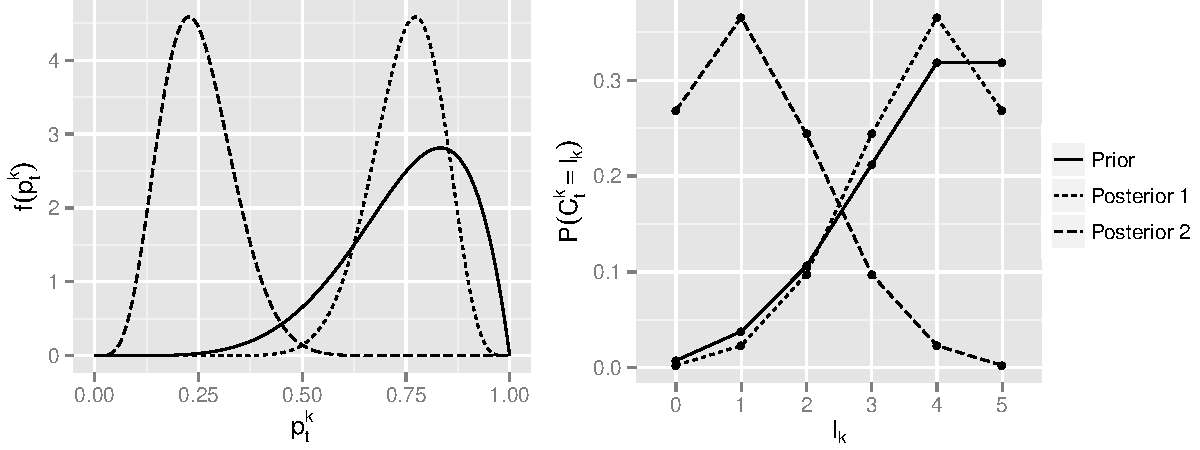
\includegraphics[width=\textwidth]{singleprior-pdc}
\caption{Beta densities (left) and corresponding Beta-binomial probability mass functions (right)
for a prior with $\nktz = 8, \yktz = 0.75$,
and posteriors based on $n^k_t=16$ observations with $s^k_t=12$ (Posterior 1) and $s^k_t=0$ (Posterior 2), respectively.
For Posterior 2, the conflict between prior assumptions and data is averaged out;
both posterior density and posterior predictive have the same spread as Posterior 1 for which there is no conflict,
giving a false sense of certainty.}
\label{fig:singleprior-pdc}
\end{figure}

 
\td{***Illustration of such prior-data conflict with $\bebin$ distribution:
different priors updated to same posterior,
or same prior updated to different posteriors with same variance,
show corresponding $C^k_t$ distribution.***}



\section{Sets of Beta Priors}

As was shown in \citet{2009:WalterAugustin}, %Walter \& Augustin (2009),
we can have both tractability and meaningful reaction to prior-data conflict
by using sets of priors $\MktZ$ produced by parameter sets $\PktZ = [\nktzl, \nktzu] \times [\yktzl, \yktzu]$. 
(A detailed discussion of different choices for $\PktZ$ is given in \citet[\S 3.1]{2013:diss-gw}.)
In our model, each prior parameter pair $(\nktz, \yktz) \in \PktZ$
corresponds to a Beta prior, thus $\MktZ$ is a set of Beta priors.
The set of posteriors $\MktN$ is obtained by updating each prior in $\MktZ$ according to Bayes' Rule.
Due to conjugacy, $\MktN$ is a set of Beta distributions with parameters $(\nktn, \yktn)$
obtained from updating $(\nktz, \yktz) \in \PktZ$ according to \eqref{eq:nyupdate},
and so can be described efficiently through the set of updated parameters
\begin{align*}
\PktN &= \Big\{ (\nktn, \yktn) \mid (\nktz, \yktz) \in \PktZ = [\nktzl, \nktzu] \times [\yktzl, \yktzu] \Big\}\,.
\end{align*}
Such rectangular prior parameter sets $\PktZ$ have been shown
to balance desirable model properties and ease of elicitation quite well.
%
For each component type $k$ and time point $t$,
one has to choose only the four parameters $\nktzl, \nktzu, \yktzl, \yktzu$
(so $4 \times |{\cal T}|$ parameters are needed to define the set of prior distributions characterizing
prior knowledge on the survival function of components of type $k$);
notwithstanding this, the model has favourable inference properties.

Central to these inference properties is that
while the prior parameter set $\PktZ$ is rectangular,
the posterior parameter set $\PktN$ is not rectangular anymore;
indeed, the shape of $\PktN$ depends on the presence of prior-data conflict,
which is naturally operationalized as $s^k_t/n^k_t \not\in [\yktzl, \yktzu]$:
prior-data conflict is present when the observed fraction of functioning components
is outside its expected range.

In absence of prior-data conflict, 
$\PktN$ shrinks in the $\ykt$ dimension;
how much it shrinks depends on $\nktz \in [\nktzl, \nktzu]$,
leading to the so-called spotlight shape depicted in Figure***.
As $\yktn$ gives the posterior expectation for the functioning probability $p_t^k$,
shorter $\yktn$ intervals mean more precise knowledge about $p_t^k$.
Also, the variance interval for $p_t^k$ will decrease
as the Beta distributions in $\MktN$ will be more pointed
due to the increase of $\nktz$ to $\nktn$.s

In case of prior-data conflict ($s^k_t/n^k_t \not\in [\yktzl, \yktzu]$),
$\PktN$ has instead the so-called banana shape,
arising from $\yktn$ intervals being shifted closer towards $s^k_t/n^k_t$
for lower $\nktn$ values than for higher $\nktn$ values, see Figure***.
Overall, this results in a wider $\yktn$ interval as compared to the non-conflict case, 
reflecting the extra uncertainty due to prior-data conflict,
thus making more cautious probability statements about $p_t^k$.

Furthermore, with sets of Beta priors it is also possible
to express prior ignorance in a more adequate way,
by letting $\yktzl \to 0$ and $\yktzu \to 1$
for some or all $t \in {\cal T}$.
(It is not advisable to choose $\yktzl = 0$ and $\yktzu = 1$,
as this can lead to improper posterior predictive distributions.
E.g., for any $t < \min(\vec{t}^k)$,
we would get $\yktnu = 1$, leading to one argument of the Beta function
in the denominator of \eqref{eq:postpredCny} being zero.)
Choosing these limits for $\yktz$ means that we are prepared to give trivial bounds for the functioning probability only,
and do not wish to make any commitments about $p^k_t$ a priori.
Compare this to the uniform prior over $[0,1]$, a usual choice of `noninformative' prior,
being a Beta prior with $\alpha^k_t = \beta^k_t = 1$, i.e., $\nktz = 2$, $\yktz = 0.5$.
Taking this for all $t \in {\cal T}$ means that we expect the component reliability function
to be on average 1/2 for all $t$, a very peculiar assumption,
and, in our view, quite incompatible with the notion of prior ignorance.

In this near-noninformative setting, the choice of $\nktzl$ not relevant,
as both $\yktnl$ and $\yktnu$ are obtained with $\nktzu$;
indeed $\yktzl > 0$ and $\yktzu < 1$ can be chosen such that
$\frac{s^k_t}{n_k} \in [\yktzl, \yktzu]$ for all $t \in \big(\min(\vec{t}^k), \max(\vec{t}^k)\big)$.
Logically, one cannot have prior-data conflict in case of prior near ignorance.

\td{***called near-noninformative, for near-noninformative sets when $\yz$ is not bounded see
benavoli zaffalon papers***}


\section{Sets of System Reliability Functions}

***Lower and upper bounds for $\Rsys(t)$ by min and max over $\PtZi{1}, \ldots, \PtZi{K}$.

***Monotonicity in $\yz_{k,t}$, so we get, for each $t \in {\cal T}$,
\begin{align*}
\lefteqn{\lRsys(t \mid \vec{t}^1, \ldots, \vec{t}^K)}\\
 &= \min_{\PtZi{1}, \ldots, \PtZi{K}} \Rsys(t \mid \PtZi{1}, \ldots, \PtZi{K}, \vec{t}^1, \ldots, \vec{t}^K) \\
 &= \min_{\nz_{1,t},\ldots,\nz_{K,t}} 
    \sum_{l_1=0}^{m_1} \cdots \sum_{l_K=0}^{m_K} \Phi(l_1, \ldots, l_K)
                                                 \prod_{k=1}^K P(C^k_t = l_k \mid \yktzl, \nktz, s^k_t) \\
 &= \min_{\nz_{1,t},\ldots,\nz_{K,t}} 
    \sum_{l_1=0}^{m_1} \cdots \sum_{l_K=0}^{m_K} \Phi(l_1, \ldots, l_K) \times \\ & \hspace*{12ex}
    \prod_{k=1}^K {m_k \choose l_k} \frac{B(l_k + \nn_{k,t}\ynl_{k,t}, m_k - l_k + \nn_{k,t}(1-\ynl_{k,t}))}
                                         {B(\nn_{k,t}\ynl_{k,t}, \nn_{k,t}(1-\ynl_{k,t}))} \,.
\end{align*}

***main contribution of the paper:
set of priors thing,
guidelines on how to choose the parameters;
this is easier in terms of $(\nz, \yz)$ than in terms of $(\alpha, \beta)$***

***How to choose the sets of priors for the survival function of type $k$ components,
i.e. how to choose $\PkZi{1}, \ldots \PkZi{\tmax}$?***

***not necessary to ensure $p^k_{t_j} \ge p^k_{t_{j+1}}$ via $\yzl_{k,t_j} \ge \yzu_{k,t_{j+1}}$
as for relatively dense $t$ grids, neighbouring intervals should be able to overlap***

***Require $\yzu_{k,t_j} \ge \yzu_{k,t_{j+1}}$ and $\yzl_{k,t_j} \ge \yzl_{k,t_{j+1}}$?
What if we know, e.g., pretty much what's going on for low $t$
but want to be much more cautious for high $t$?
$\yktzl$ can then drop to 0, but are we ok that $\yktzu$ cannot increase?
(Prior guess for $p^k_t$ interpretation would say that $\yktz$ cannot increase,
but does this need to hold for the prior guess range bound $\yktzu$?)***

***generally require $\yktzl > 0$ and $\yktzu < 1$ for all $t \not\in \big(\min(\vec{t}^k), \max(\vec{t}^k)\big)$
to get proper posteriors!?!***

***what to do in extreme tail of component distributions?
How sensitive is the method to choosing prior (lower, upper) mean near-zero (how near?) for $p^k_t$ at high $t$'s?***


\section{Computations \& Examples}

***code published in Louis' \textbf{R} package \texttt{ReliabilityTheory}
(which contains the function to calculate the survival signature)***


***calculate and show $\Rsys(t)$ plots for a range of examples (keep system layout fixed?):
informative prior set for some component types, different degree of imprecision,
noninformative prior set for other components (make clear that precise `noninformative' prior actually contains info), 
combine with prior-data conflict and non-conflict test data,
to show effect of precision of prior knowledge / amount of data / (degree of) prior-data conflict on $\Rsys(t)$.***

***Vacuous prior sets $[\yktzl, \yktzu] = (0,1)$ for some component types,
informative prior sets for others. $[\nktzl, \nktzu]$ interval for all component types.***

***Some extra illustrations? E.g. the effect of extra redundancy on $\Rsys(t)$ intervals like in Risk Analysis paper?
(could nicely illustrate challenges in decision making with intervals:
do I prefer adding redundancy such that there is a chance for a large effect, but high uncertainty for it,
or do I rather add redundancy such that effect is smaller but more certain?***

***Other interesting extra illustration:
show effect of replacement of components in system at certain time points
(could be corrective (component failed) or preventive replacement),
replaced components constitute a new type with shifted component reliability function***


\section{Conclusions and Outlook}

***Extend the model to deal with right-censored observations which are common in the reliability setting.
We believe that a minimal assumption (component can fail immediately after censoring or live forever)
will be simple to implememt but will lead to high imprecision,
whereas assuming exchangeability with other surviving components at moment of censoring
will be more complex to accomodate but will lead to less imprecision.

***right-censoring will also allow to use data from running system,
to calculate its remaining useful life (RUL).



% ------------ bibliography -------------

\section*{References}

\bibliographystyle{elsarticle-harv}
\bibliography{ijar-npb-refs}

\end{document}

